\usepackage{tikz}
\usetikzlibrary{calc}
\usetikzlibrary{math}
\usetikzlibrary{decorations.pathreplacing}

\newlength{\barwidth}
\setlength{\barwidth}{0.55cm}

\newcommand{\drawaxes}[1]{
  \draw[gray]  (-.2, 0) -> (3.75 * \barwidth + .2cm, 0);
  \draw                    (3.75 * \barwidth + .2cm, 0) node[anchor=west] {$x$};
  \draw[gray]  (-.2, 0) -> (-.2, 5.2);
  \draw                    (-.2, 5.2) node[anchor=south] {$#1$};
  \foreach \x in {0.5, 1.5, 2.5, 3.5}
    \draw[gray] (\x * \barwidth, -2pt) -- (\x * \barwidth, 0pt);
  \foreach \x/\char in {0.5/a, 1.5/b, 2.5/c, 3.5/d}
    \draw (\x * \barwidth, 0) node[anchor=north, text height=8] {\texttt\char};
}

\newcommand{\ytick}[2]{% height, label
  \draw[gray] (-.2cm - 2pt, #1) node[anchor=east, color=black] {#2} -- (-.2cm + 0pt, #1);
}

\newcommand{\drawbar}[3]{
  \draw[#3] (#1, 0) -- (#1, 12.5cm * #2);
}

\newcommand{\drawpmf}{
\begin{tikzpicture}
  \drawaxes{P(x)}
  \foreach \y in {0.125, 0.25, 0.375}{\ytick{12.5 * \y}{$\y$}}
  \drawbar{0.5\barwidth}{0.125}{}
  \drawbar{1.5\barwidth}{0.25}{}
  \drawbar{2.5\barwidth}{0.375}{}
  \drawbar{3.5\barwidth}{0.25}{}
\end{tikzpicture}
}

\newcommand{\drawapprox}[2]{
\begin{tikzpicture}
  \tikzmath{
    \splus = #1 + 1;
    \yunit = 12.5 / \splus;
  }
  % \draw[xstep=\barwidth, ystep=\yunit, lightgray, very thin]
  %   (0, 0) grid (4 * \barwidth, 5.2);
    \drawaxes{s'}
  \foreach \y [parse=true, count=\s] in {\yunit, 2 * \yunit, ..., 5.2}{
    \ytick{\y}{}
    \draw (-.2cm, \y - \yunit / 2) node[anchor=east]
      {\pgfmathparse{int(\s - 1)}#2$\pgfmathresult$};
  }
  % \foreach \x/\freq/\start in {0/1/0, 1/2/1, 2/3/3, 3/2/6}{
  %   \foreach \y [parse=true, count=\s] in {\yunit, 2 * \yunit, ..., 5.2}{
  %     \tikzmath{
  %       \snew = int(8 * int((\s - 1) / \freq) + mod((\s - 1), \freq) + \start);
  %       if \snew>#1 then {\toprint = \snew;} else {let \toprint = ;};
  %       }
  %     \draw ($6.25/\splus*(0, -1) + 0.5*(\barwidth,0)
  %     + \s*(0, 12.5 / \splus) + \x*(\barwidth, 0)$)
  %     node [text=lightgray] {#2$\toprint$};
  %   }
  % }
  % \drawbar{0\barwidth}{0.125}{thin, gray}
  % \drawbar{1\barwidth}{0.25} {thin, gray}
  % \drawbar{2\barwidth}{0.375}{thin, gray}
  % \drawbar{3\barwidth}{0.25} {thin, gray}
  \foreach \x/\freq/\start in {0/1/0, 1/2/1, 2/3/3, 3/2/6}{
    \foreach \y [parse=true, count=\s] in {\yunit, 2 * \yunit, ..., 5.2}{
      \tikzmath{
        \snew = int(8 * int((\s - 1) / \freq) + mod((\s - 1), \freq) + \start);
        if \snew<=#1 then {\toprint = \snew;} else {let \toprint = ;};
        }
      \draw ($(0, -\yunit / 2) + 0.5*(\barwidth,0)
      + \s*(0, \yunit) + \x*(\barwidth, 0)$) node {#2$\toprint$};
    }
  }
\end{tikzpicture}
}

\newlength{\intervalwidth}
\setlength{\intervalwidth}{0.7\textwidth}

\newlength{\gap}
\setlength{\gap}{0.15cm}

\newlength{\lineheight}
\setlength{\lineheight}{0.45cm}
\newcommand{\drawinterval}{
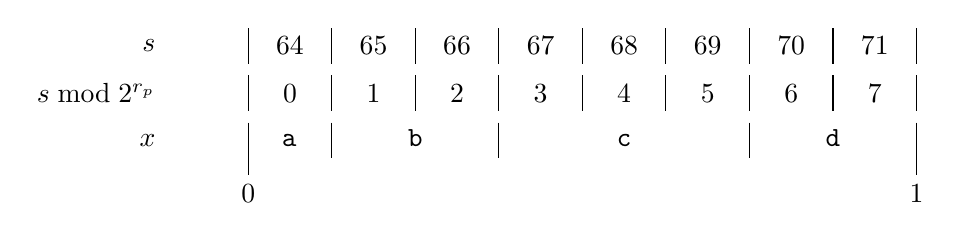
\begin{tikzpicture}
  \draw (-30pt, 0) node [anchor=east] {$s$};
  \draw (0, -.5\lineheight) -- (0, .5\lineheight);
  \draw (\intervalwidth, -.5\lineheight) -- (\intervalwidth, .5\lineheight);
  \foreach \s in {1, ..., 7}{
    \draw (\s * 0.125 * \intervalwidth, -.5\lineheight)
      -- (\s * 0.125 * \intervalwidth, .5\lineheight);
  }
  \foreach \y in {0, ..., 7}{
    \tikzmath{
      \x = (\y * 0.125 + 0.0625);
      \r = int(\y + 64);
    }
    \draw (\x\intervalwidth, 0) node {$\r$};
  }

  \draw (-30pt, -\lineheight -\gap) node [anchor=east] {$s \bmod 2^{r_p}$};
  \draw (0, -.5\lineheight - \gap) -- (0, -1.5\lineheight -\gap);
  \draw (\intervalwidth, -.5\lineheight - \gap)
    -- (\intervalwidth, -1.5\lineheight - \gap);
  \foreach \s in {1, ..., 7}{
    \draw (\s * 0.125 * \intervalwidth, -.5\lineheight - \gap)
      -- (\s * 0.125 * \intervalwidth, -1.5\lineheight - \gap);
  }
  \foreach \s in {0, ..., 7}{
    \tikzmath{
      \x = (\s * 0.125 + 0.0625);
    }
    \draw (\x\intervalwidth, -\lineheight - \gap) node  {$\s$};
  }

  \draw (-30pt, -2\gap - 2\lineheight) node [anchor=east] {$x$};
  \draw (0, -2\gap - 1.5\lineheight) -- (0, -2\gap - 2.5\lineheight - 6pt);
  \draw (\intervalwidth, -2\gap - 1.5\lineheight)
    -- (\intervalwidth, -2\gap - 2.5\lineheight - 6pt);
  \draw (0, -2\gap - 2.5\lineheight - 6pt) node [anchor=north] {$0$};
  \draw (\intervalwidth, -2\gap - 2.5\lineheight - 6pt) node [anchor=north] {$1$};
  \draw (0.125  \intervalwidth, -2\gap - 1.5\lineheight)
    -- (0.125 * \intervalwidth, -2\gap - 2.5\lineheight);
  \draw (0.375  \intervalwidth, -2\gap - 1.5\lineheight)
    -- (0.375 * \intervalwidth, -2\gap - 2.5\lineheight);
  \draw (0.75  \intervalwidth, -2\gap - 1.5\lineheight)
    -- (0.75 * \intervalwidth, -2\gap - 2.5\lineheight);
  \draw (0.06125\intervalwidth, -2\gap - 2\lineheight)
    node [text height=1ex] {\texttt{a}};
  \draw (0.25   \intervalwidth, -2\gap - 2\lineheight)
    node [text height=1ex] {\texttt{b}};
  \draw (0.5625 \intervalwidth, -2\gap - 2\lineheight)
    node [text height=1ex] {\texttt{c}};
  \draw (0.875  \intervalwidth, -2\gap - 2\lineheight)
    node [text height=1ex] {\texttt{d}};

\end{tikzpicture}
}


\newlength{\tbase}
\setlength{\tbase}{-0cm}


\newcommand{\drawmessage}{
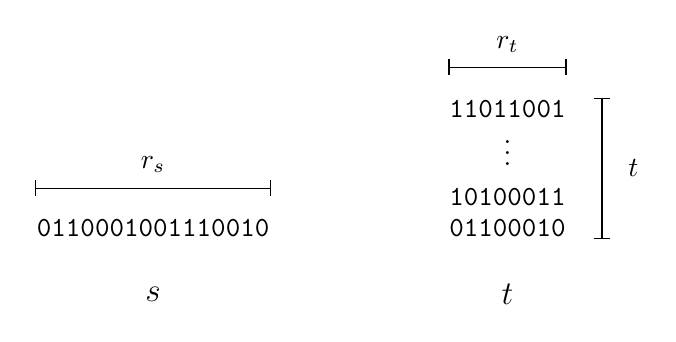
\begin{tikzpicture}
  \node at (0, 0) (s) {\texttt{0110001001110010}};
  % \draw [decorate,decoration={brace,amplitude=5pt,mirror}]
  %   (-1.46, -0.4) -- (1.46, -0.4);
  \node at (0, -0.85) {\large\(s\)};
  \draw [{|-|}] (-1.5, 0.5) -- (1.5, 0.5);
  \node at (0, 0.8) {\(r_s\)};

  \node at (4.5, \tbase) {\texttt{01100010}};
  \node at (4.5, \tbase + 11) {\texttt{10100011}};
  \node at (4.5, \tbase + 30) {\(\vdots\)};
  \node at (4.5, \tbase + 43) {\texttt{11011001}};
  \draw [{|-|}] (4.5 - 0.75, \tbase + 58) -- (4.5 + 0.75, \tbase + 58);
  \node at (4.5, \tbase + 66) {\(r_t\)};
  % \draw [decorate,decoration={brace,amplitude=5pt,mirror}]
  %   (4.5 - 0.75, \tbase - 0.4cm) -- (4.5 + 0.75, \tbase - 0.4cm);
  \node at (4.5, -0.85) {\large\(t\)};
  \draw [{|-|}] (4.5 + 1.2, \tbase - 4) -- (4.5 + 1.2, \tbase + 43 + 4);
  \node at (4.5 + 1.6, \tbase + 21.5) {\(\abs{t}\)};
\end{tikzpicture}
}
